\documentclass[aspectratio=169,10pt]{beamer}

% ============================================================
% Hybrid Quantum AI for Multiphysics Simulation -- seminar deck
% Madrid theme, 5 sections. Figures live in figures/.
% Compile: latexmk -pdf qiskit_hybrid_quantum_ai.tex
% ============================================================

\usetheme{Madrid}
\usecolortheme{seahorse}

\usepackage[utf8]{inputenc}
% \usepackage[T1]{fontenc}
\usepackage{amsmath,amssymb}
\usepackage{booktabs}
\usepackage{graphicx}
\usepackage[export]{adjustbox}
\usepackage{xcolor}
\usepackage{tikz}
\usetikzlibrary{arrows.meta,decorations.pathmorphing}
\graphicspath{{figures/}}

\setbeamertemplate{navigation symbols}{}

\definecolor{qpurple}{HTML}{6B4C9A}
\definecolor{cblue}{HTML}{2C6E9E}
\definecolor{okgreen}{HTML}{2E7D4F}
\definecolor{warnorange}{HTML}{C9731C}
\definecolor{qred}{HTML}{B03A2E}
\definecolor{phgray}{HTML}{6E7780}

% Equation that shrinks only if wider than the text
\newcommand{\eq}[1]{\[\adjustbox{max width=0.94\linewidth}{$\displaystyle #1$}\]}

% One-line message at the bottom of a slide
\newcommand{\takeaway}[1]{%
  \vfill
  \begin{beamercolorbox}[rounded=true,shadow=false,wd=\linewidth,sep=4pt]{block title}
  \small\centering #1
  \end{beamercolorbox}}

% Figure caption line
\newcommand{\figcap}[1]{\par\vspace{1pt}{\scriptsize\color{phgray}#1\par}}

\title[Hybrid Quantum AI for Multiphysics]{Hybrid Quantum AI Models for Accelerating\\Multiphysics Simulation- Part 1}
\subtitle{For Crystal Growth Simulations and Liquid H$_2$ Cryogenics}
%\subtitle{QISKIT Seminar}
\author{Quasi Team, Collaborators} 
\date{October 2026}

\begin{document}

\begin{frame}
\titlepage
\end{frame}

\begin{frame}{Outline}
\tableofcontents
\end{frame}

% =====================================================================
\section{Motivation}
% =====================================================================

\begin{frame}{Multiphysics simulation is too slow for design loops}
\begin{columns}[T,onlytextwidth]
\column{0.56\textwidth}
\begin{itemize}\small\setlength{\itemsep}{3pt}
  \item High-fidelity coupled CFD (flow + heat + rotation + phase change) takes hours to days per run.
  \item Every new operating point (heater power, rotation rate, fill level) is a new simulation.
  \item Process control and digital twins need full fields in \textbf{milliseconds}.
\end{itemize}
\vspace{0.1cm}
\begin{block}{Goal}
\small A surrogate that keeps the governing physics, generalises across operating conditions, and evaluates in real time.
\end{block}
\column{0.40\textwidth}
\centering
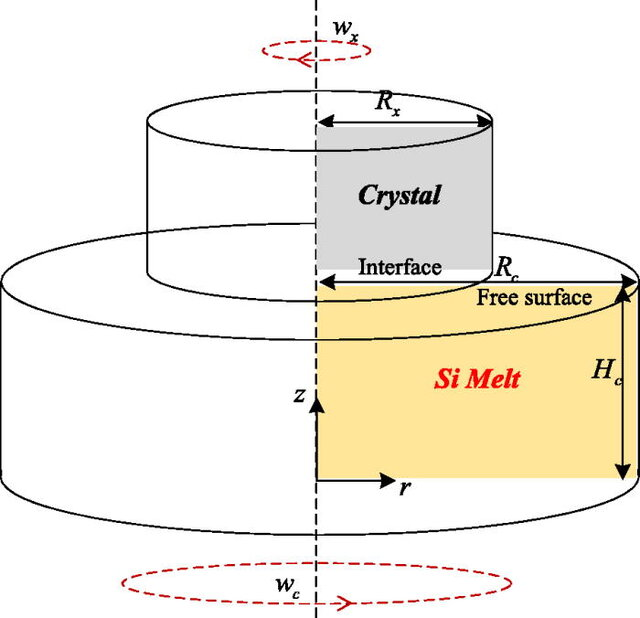
\includegraphics[width=\linewidth,height=0.56\textheight,keepaspectratio]{Simulation-region-of-silicon-single-crystal-growth_W640.jpg}
\figcap{Czochralski (CZ) growth: crystal rotating at $\omega_s$, pulled from a Si melt in a crucible rotating at $\omega_c$.}
\end{columns}
\takeaway{Accuracy is not the key bottleneck; the design space.}
\end{frame}

\begin{frame}{Two industrial use cases}
\begin{columns}[T,onlytextwidth]
\column{0.58\textwidth}
\begin{block}{Silicon crystal growth (Czochralski)}
\footnotesize Melt convection, swirl and temperature (1685--1750\,K) set defect density and oxygen uptake. Five coupled fields per point: $u_r,u_z,u_\theta,p,T$.
\end{block}
\vspace{0.05cm}
\centering
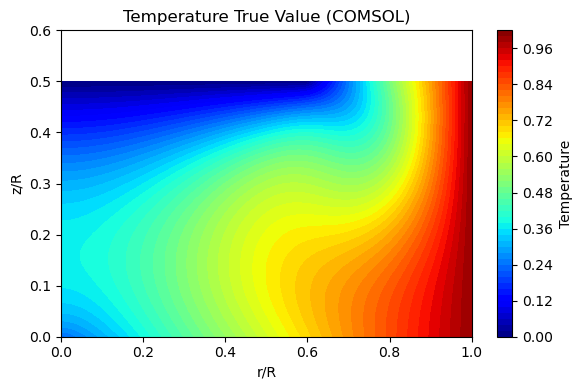
\includegraphics[width=0.49\linewidth]{temp.png}\hfill
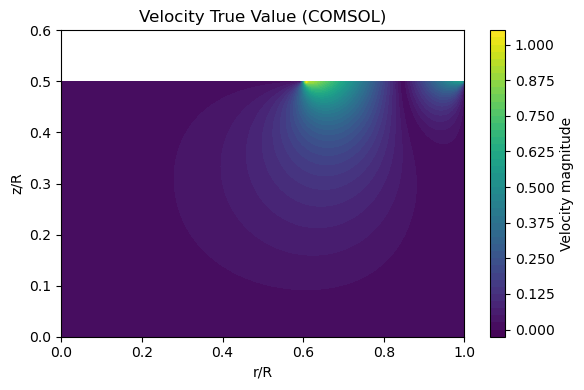
\includegraphics[width=0.49\linewidth]{velocity.png}
\figcap{COMSOL reference: temperature (left) and velocity magnitude (right). Sharp gradients sit at the free surface and the crystal edge.}
\column{0.38\textwidth}
\begin{block}{LH$_2$ cryogenic boil-off}
\begin{itemize}\footnotesize
  \item Heat leak into liquid-hydrogen tanks ($\approx$20\,K) drives natural convection, stratification and evaporation.
  \item Turbulent convection with a \textbf{moving liquid--vapour interface}.
  \item Aim: boil-off rate and pressure rise for tank design.
\end{itemize}
\end{block}
\begin{exampleblock}{Common thread}
\footnotesize Strongly coupled, non-linear transport of velocity, temperature, species and interfaces.
\end{exampleblock}
\end{columns}
\end{frame}

\begin{frame}{Key ideas}
\begin{enumerate}\setlength{\itemsep}{5pt}
  \item \textbf{Problem:} classical PINNs suffer from spectral bias, loss imbalance and badly scaled coupled fields.
  \item \textbf{Model:} Hybrid-QPINN / QPINO: a classical network with a shallow parameterised quantum circuit (PQC) as a trainable feature map, fed by Fourier features and data re-uploading.
  \item \textbf{Tools:} PennyLane (training), Qiskit Aer (simulation), Qiskit Runtime (IBM hardware).
  \item \textbf{Benchmarks:} silicon CZ crystal growth (running) and LH$_2$ boil-off (defined).
  \item \textbf{Destination:} real-time digital twins and fast parametric exploration.
\end{enumerate}
\takeaway{Goal: Hybrid quantum surrogates that answer in milliseconds instead of hours.}
\end{frame}

% =====================================================================
\section{Classical approaches}
% =====================================================================

\begin{frame}{Physics-informed neural networks (PINNs)}
\begin{columns}[T,onlytextwidth]
\column{0.54\textwidth}
\centering
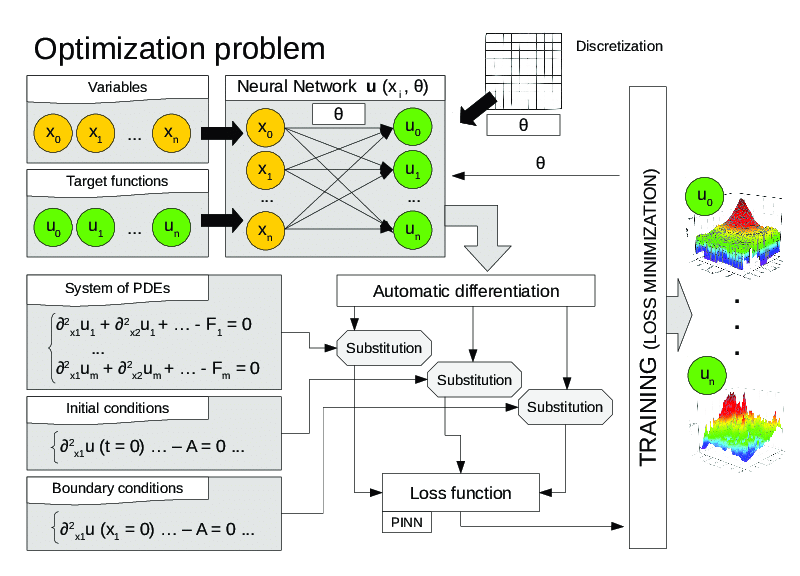
\includegraphics[width=\linewidth,height=0.60\textheight,keepaspectratio]{pinns_2.png}
\figcap{Inputs $\to$ network $\to$ automatic differentiation $\to$ PDE, IC and BC residuals $\to$ loss $\to$ training.}
\column{0.43\textwidth}
\begin{enumerate}\small\setlength{\itemsep}{2pt}
  \item A network $u(x,\theta)$ maps coordinates to the target fields.
  \item Automatic differentiation gives exact derivatives, so PDE residuals can be evaluated at any point: no mesh.
  \item Residuals of PDEs, initial and boundary conditions are combined into one loss:
\end{enumerate}
\eq{\mathcal L=\lambda_{\mathrm{PDE}}\mathcal L_{\mathrm{PDE}}+\lambda_{\mathrm{IC}}\mathcal L_{\mathrm{IC}}+\lambda_{\mathrm{BC}}\mathcal L_{\mathrm{BC}}\,(+\,\mathcal L_{\mathrm{data}})}
\begin{alertblock}{Limits}
\footnotesize One trained PINN = one operating point (Neüral Operator learns familie of fünctions). The weights $\lambda$ decide what is actually learned.
\end{alertblock}
\end{columns}
%\takeaway{Physics enters through the loss, so little labelled data is needed; three bottlenecks follow.}
\end{frame}

\begin{frame}{Bottleneck 1: spectral bias}
\begin{columns}[T,onlytextwidth]
\column{0.42\textwidth}
\begin{itemize}\small\setlength{\itemsep}{3pt}
  \item Neural networks learn low frequencies first; sharp content converges slowly (Rahaman et al., 2019).
  \item Transport fields are full of sharp structure: thermal boundary layers, swirl near rotating walls, phase interfaces.
  \item Classical remedy: Fourier feature inputs (Tancik et al., 2020).
\end{itemize}
\column{0.56\textwidth}
\centering
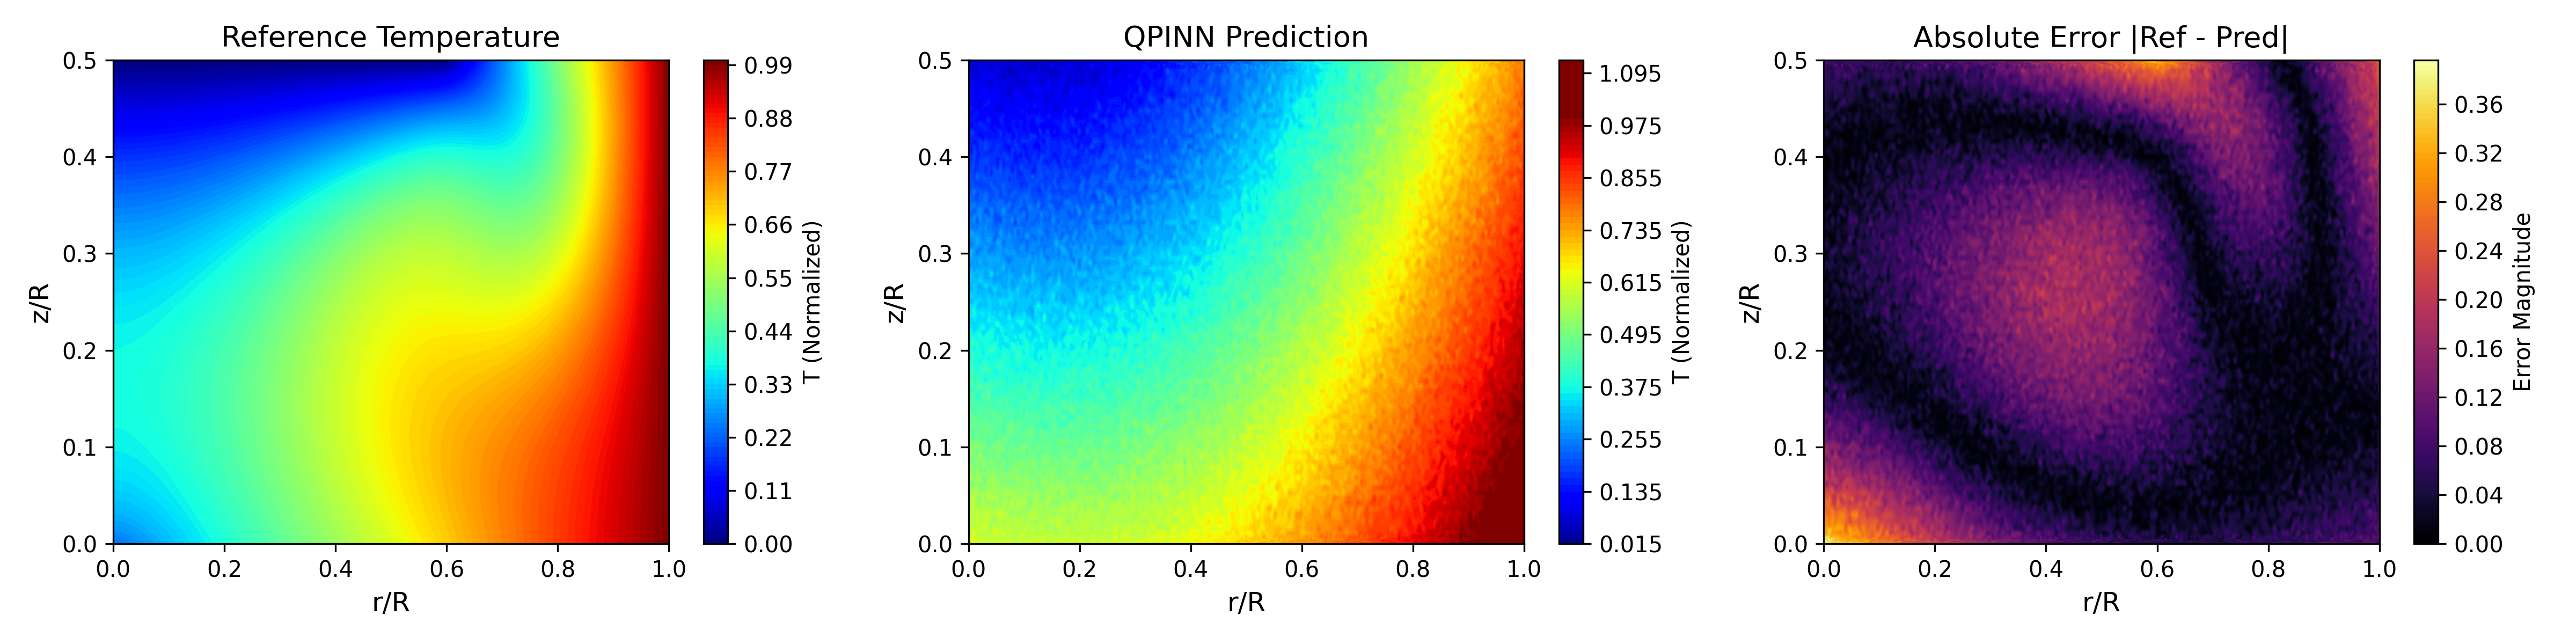
\includegraphics[width=\linewidth]{qpinn_comparison_error.png}
\figcap{Reference temperature, a smooth network prediction and the absolute error, which concentrates on the curved thermal front.}
\end{columns}
\takeaway{Errors live where the physics is sharpest: the part of the field design decisions depend on.}
\end{frame}

\begin{frame}{Classical PINN on simplified crystal growth}
\begin{columns}[T,onlytextwidth]
\column{0.38\textwidth}
\centering
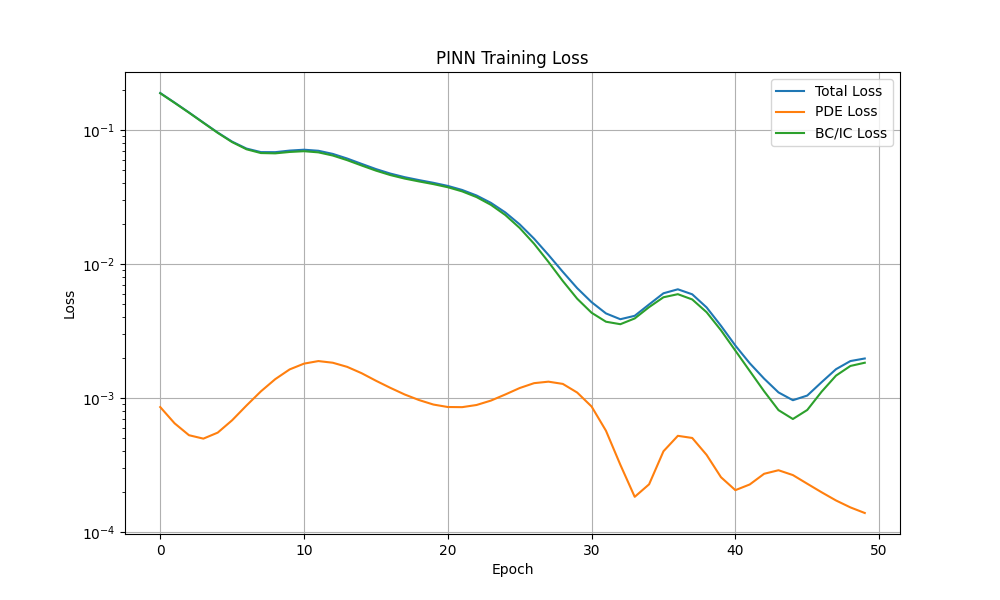
\includegraphics[width=\linewidth]{crystal_growth_loss.png}
\figcap{Training loss: total, PDE and BC/IC components.}
\begin{itemize}\footnotesize
  \item Total loss follows BC/IC; the PDE term oscillates instead of falling.
  \item Loss rises again after epoch 45.
\end{itemize}
\column{0.60\textwidth}
\centering
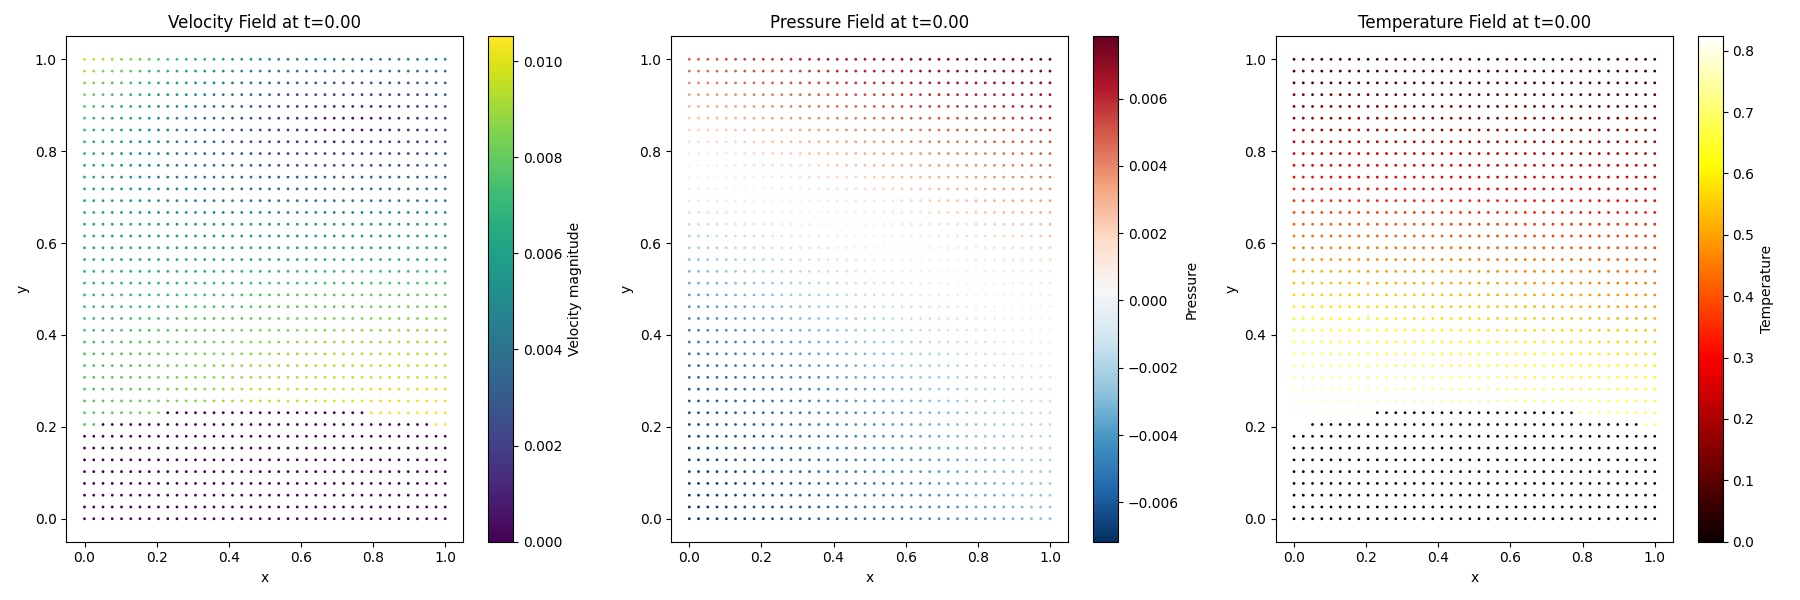
\includegraphics[width=0.92\linewidth]{crystal_growth_t0_0.png}\\[-1pt]
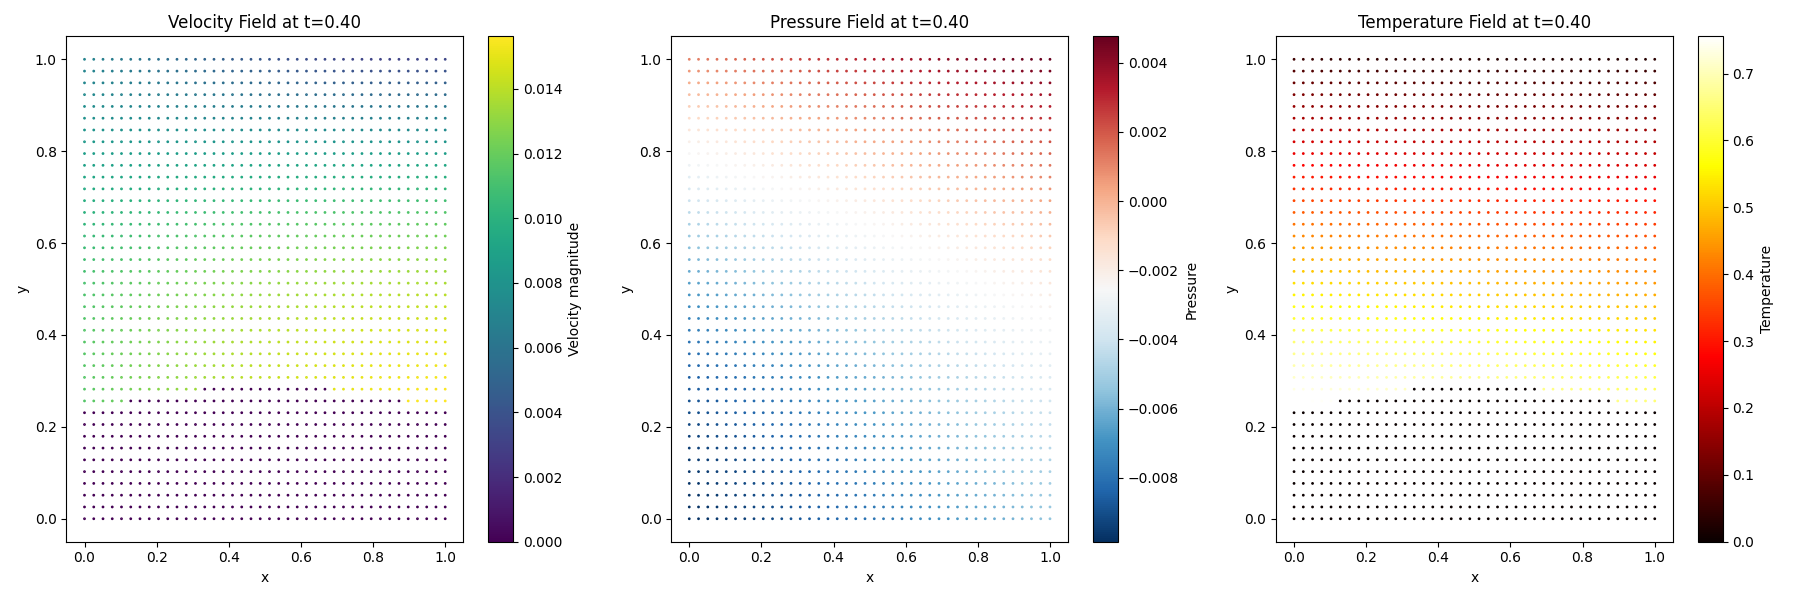
\includegraphics[width=0.92\linewidth]{crystal_growth_t0_4.png}
\figcap{Predicted velocity, pressure and temperature at $t=0$ (top) and $t=0.4$ (bottom).}
\end{columns}
\takeaway{A plain PINN converges to smooth, under-resolved fields.}
\end{frame}

\begin{frame}{Bottleneck 2: loss-term imbalance}
\begin{columns}[T,onlytextwidth]
\column{0.50\textwidth}
\begin{center}
\footnotesize
\begin{tabular}{lccc}
\toprule
Trainer (1D heat) & PDE loss & BC/IC loss & Rel.\ $L_2$ \\
\midrule
Baseline    & $3.96\!\times\!10^{-3}$ & $1.15\!\times\!10^{-3}$ & $0.084$ \\
GNPINN      & $9.74\!\times\!10^{-3}$ & $\mathbf{9.05\!\times\!10^{-4}}$ & $\mathbf{0.054}$ \\
AgenticPINN & $\mathbf{8.22\!\times\!10^{-7}}$ & $2.00\!\times\!10^{-1}$ & \textcolor{qred}{$\mathbf{1.368}$} \\
\bottomrule
\end{tabular}
\end{center}
\begin{itemize}\footnotesize
  \item Baseline: fixed weights. GNPINN: gradient-normalised. AgenticPINN: rule-based re-weighting.
  \item AgenticPINN: PDE residual $\approx$4800$\times$ smaller, BC/IC $\approx$173$\times$ larger, and the solution is wrong.
\end{itemize}
\column{0.47\textwidth}
\centering
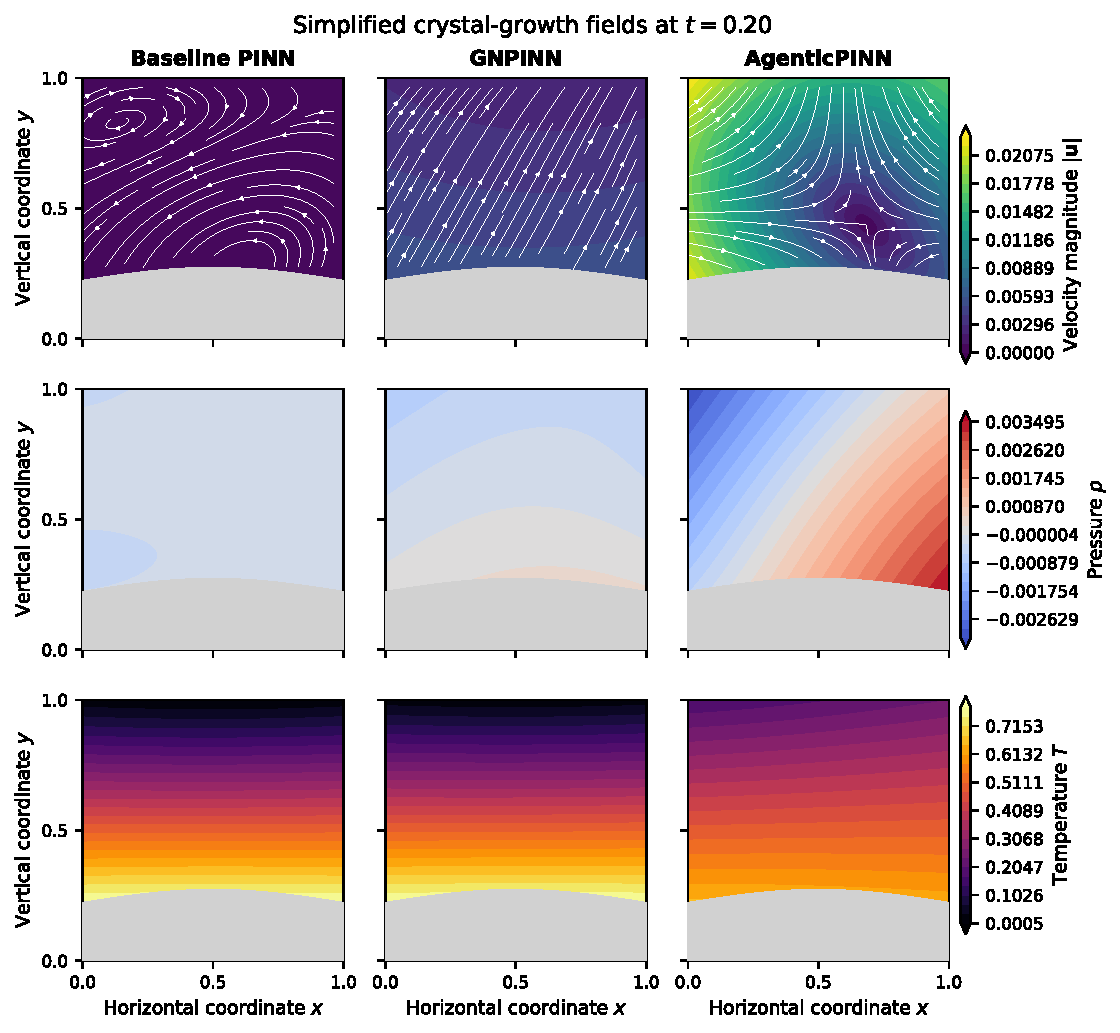
\includegraphics[width=\linewidth,height=0.66\textheight,keepaspectratio]{crystal_mlp_fields.pdf}
\figcap{Simplified CZ fields at $t=0.2$ for the three trainers (Chapagain et al., 2026).}
\end{columns}
\takeaway{The smallest PDE loss gave the worst solution: always report per-term and per-field errors.}
\end{frame}

\begin{frame}{Bottleneck 3: scale mismatch between coupled fields}
\begin{columns}[T,onlytextwidth]
\column{0.55\textwidth}
\begin{itemize}
  \item Five outputs $u_r, u_z, u_\theta, p, T$ with very different magnitudes.
  \item In the CZ model the pressure coefficient is
  \[p_{\mathrm{coeff}} = \frac{p_{\mathrm{scale}}}{v_{\mathrm{scale}}^2} = 134{,}128,\]
  while viscous terms scale as $1/Re \approx 0.067$.
  \item Pressure-to-viscous ratio $\approx 2\times10^{6}:1$.
\end{itemize}
\column{0.41\textwidth}
\begin{alertblock}{Consequence}
The pressure residual can swamp the data signal during physics-informed training (Result 4).
\end{alertblock}
\vspace{0.2cm}
\begin{block}{Design response}
Hard constraints, staged physics warm-up, residual balancing, per-field residual scaling.
\end{block}
\end{columns}
\takeaway{Non-dimensionalisation is part of the model, not a pre-processing detail.}
\end{frame}

% =====================================================================
\section{Hybrid quantum--classical model}
% =====================================================================

\begin{frame}{Architecture overview}
\centering
\resizebox{\linewidth}{!}{%
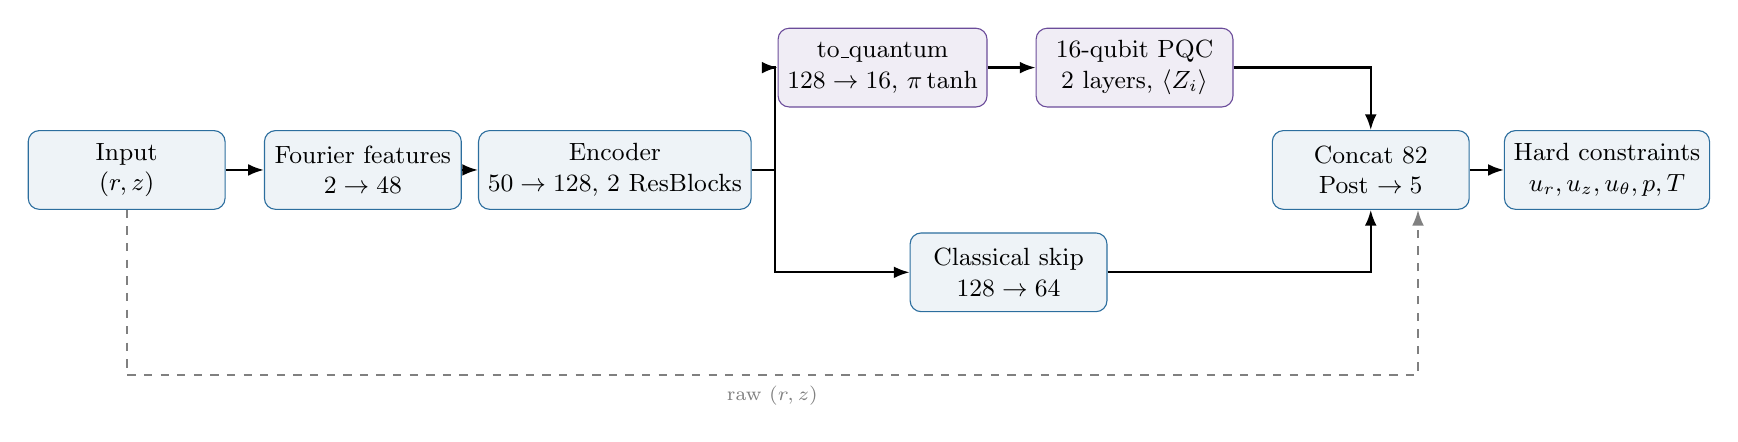
\begin{tikzpicture}[
  font=\small,
  cls/.style={rounded corners,draw=cblue,fill=cblue!8,minimum height=1.0cm,minimum width=2.5cm,align=center},
  qnt/.style={rounded corners,draw=qpurple,fill=qpurple!10,minimum height=1.0cm,minimum width=2.5cm,align=center},
  arr/.style={-{Latex[length=2mm]},thick}
]
\node[cls] (in) at (0,0) {Input\\$(r,z)$};
\node[cls] (ff) at (3.0,0) {Fourier features\\$2\to48$};
\node[cls] (enc) at (6.2,0) {Encoder\\$50\to128$, 2 ResBlocks};
\node[qnt] (tq) at (9.6,1.3) {to\_quantum\\$128\to16$, $\pi\tanh$};
\node[qnt] (pqc) at (12.8,1.3) {16-qubit PQC\\2 layers, $\langle Z_i\rangle$};
\node[cls] (sk) at (11.2,-1.3) {Classical skip\\$128\to64$};
\node[cls] (post) at (15.8,0) {Concat 82\\Post $\to5$};
\node[cls] (out) at (18.8,0) {Hard constraints\\$u_r,u_z,u_\theta,p,T$};
\draw[arr] (in)--(ff); \draw[arr] (ff)--(enc);
\draw[arr] (enc.east)--++(0.3,0)|-(tq.west);
\draw[arr] (enc.east)--++(0.3,0)|-(sk.west);
\draw[arr] (tq)--(pqc);
\draw[arr] (pqc.east)-|(post.north);
\draw[arr] (sk.east)-|(post.south);
\draw[arr] (post)--(out);
\draw[arr,dashed,gray] (in.south)--++(0,-2.1)-|node[pos=0.25,below,font=\scriptsize]{raw $(r,z)$} ([xshift=0.6cm]post.south);
\end{tikzpicture}}

\vspace{0.2cm}
\begin{columns}[T,onlytextwidth]
\column{0.32\textwidth}
\begin{block}{Classical backbone}
\footnotesize Fourier encoding + residual MLP + post network: 125,925 parameters.
\end{block}
\column{0.32\textwidth}
\begin{exampleblock}{Quantum feature map}
\footnotesize 16 qubits, 2 layers: \textbf{96} trainable angles (0.076\% of 126,021).
\end{exampleblock}
\column{0.32\textwidth}
\begin{block}{Skip path}
\footnotesize 64 classical features bypass the PQC, so the head never depends solely on it.
\end{block}
\end{columns}
\takeaway{The PQC is a small, expressive feature extractor; the classical network does the heavy lifting.}
\end{frame}

\begin{frame}{Ingredient 1: Fourier feature mapping}
\begin{columns}[T,onlytextwidth]
\column{0.54\textwidth}
\begin{itemize}\small
  \item Frozen random matrix $B\in\mathbb{R}^{2\times24}$, $B_{ij}\sim\mathcal{N}(0,6^2)$:
  \eq{\gamma(x) = \big[\sin(2\pi\,xB),\ \cos(2\pi\,xB)\big]\in\mathbb{R}^{48}}
  \item Frequencies up to roughly $\pm15$ cycles per unit length.
  \item Concatenated with raw $(r,z)$: 50 encoder inputs.
  \item High-frequency access from the first layer at zero trainable cost.
\end{itemize}
\column{0.42\textwidth}
\centering
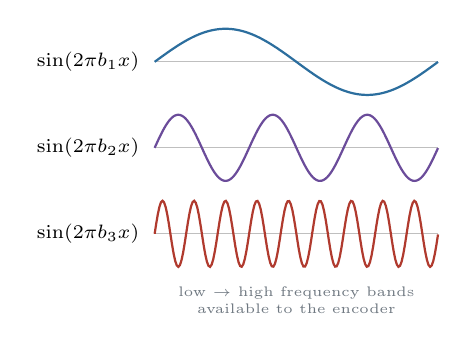
\begin{tikzpicture}[x=3.6cm,y=0.42cm,font=\scriptsize]
\foreach \f/\yo/\c [count=\i] in {1/0/cblue,3/-2.6/qpurple,9/-5.2/qred}{
  \draw[gray!50] (0,\yo)--(1,\yo);
  \draw[thick,\c,domain=0:1,samples=180] plot (\x,{\yo+sin(\f*360*\x)});
  \node[anchor=east] at (-0.02,\yo) {$\sin(2\pi b_{\i}x)$};
}
\node[font=\tiny,text=phgray,align=center] at (0.5,-7.2) {low $\rightarrow$ high frequency bands\\available to the encoder};
\end{tikzpicture}
\end{columns}
\takeaway{Fourier features fix the input spectrum; the PQC adds a trainable spectrum deeper in the network.}
\end{frame}

\begin{frame}{Ingredient 2: shallow parameterised quantum circuit}
\begin{columns}[T,onlytextwidth]
\column{0.46\textwidth}
\centering
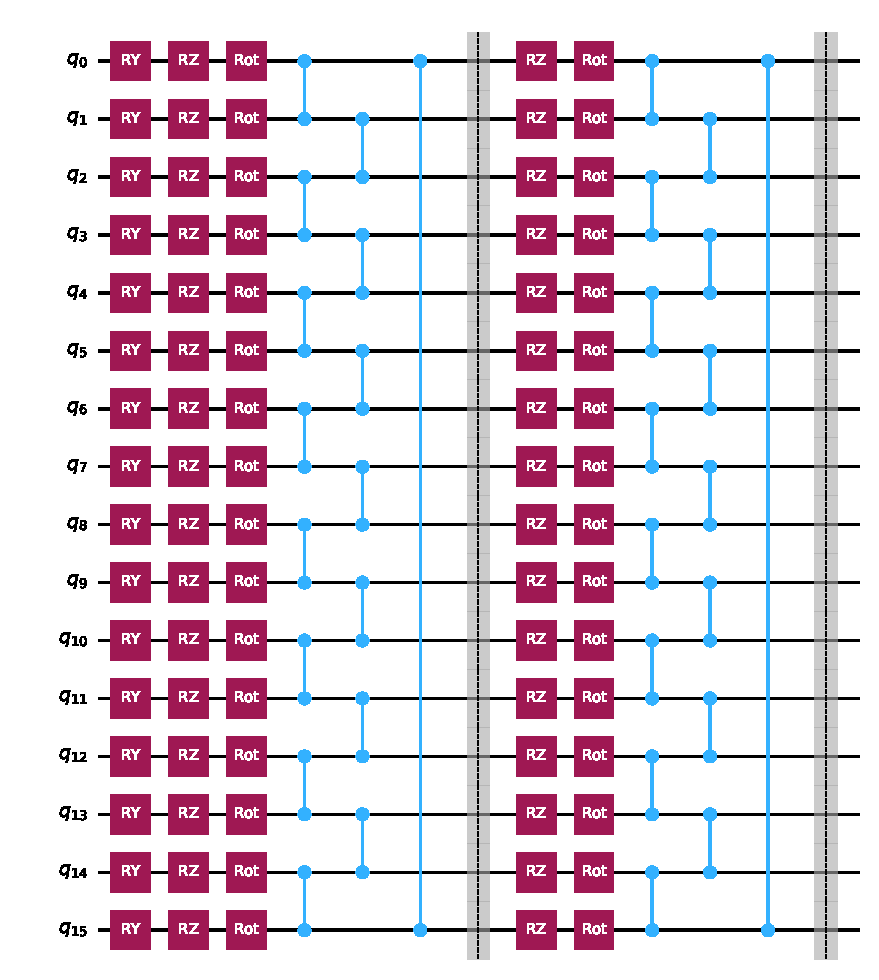
\includegraphics[width=\linewidth,height=0.64\textheight,keepaspectratio]{circuit_logical.pdf}
\figcap{Logical circuit: 16 qubits, 2 layers, CZ ring.}
\column{0.51\textwidth}
\begin{enumerate}\small\setlength{\itemsep}{1pt}
  \item \textbf{Encode:} $R_Y(\theta_i)$, $\theta_i=\pi\tanh(h_i)\in[-\pi,\pi]$.
  \item \textbf{Re-upload} (each layer $\ell$): $R_Z(0.5\,\theta_{(i+\ell)\bmod16})$.
  \item \textbf{Train:} $\mathrm{Rot}(\varphi,\vartheta,\omega)=R_Z R_Y R_Z$, 48 angles/layer.
  \item \textbf{Entangle:} CZ ring $q_0$--$q_1$--$\cdots$--$q_{15}$--$q_0$.
  \item \textbf{Read out:} $\langle Z_i\rangle\in[-1,1]$ $\to$ LayerNorm(16).
\end{enumerate}
\vspace{0.1cm}
\begin{center}
\footnotesize
\begin{tabular}{lr@{\hspace{1.2em}}lr}
\toprule
$R_Y$ (encode) & 16 & CZ (entangle) & 32 \\
$R_Z$ (re-upload) & 32 & Total gates & 112 \\
Rot (trainable) & 32 & Logical depth & 9 \\
\bottomrule
\end{tabular}
\end{center}
\end{columns}
\takeaway{Only 32 two-qubit gates: shallow enough to run reliably on today's hardware.}
\end{frame}

\begin{frame}{Ingredient 3: data re-uploading}
\begin{columns}[T,onlytextwidth]
\column{0.56\textwidth}
\begin{itemize}\small\setlength{\itemsep}{2pt}
  \item A PQC output is a truncated Fourier series of its encoded inputs (Schuld et al., 2021):
  \eq{f_\Phi(\theta) = \sum_{\omega\in\Omega} c_\omega(\Phi)\, e^{i\omega\cdot\theta}}
  \item Encoding gates fix the frequencies $\Omega$; trainable gates set the coefficients $c_\omega$.
  \item Each $\theta_i$ enters three times ($R_Y$ once, $R_Z(\tfrac12\theta)$ twice), and the cyclic shift mixes neighbouring latent features in each layer.
\end{itemize}
\column{0.40\textwidth}
\begin{center}
\footnotesize
\begin{tabular}{lc}
\toprule
Encoding of $\theta_i$ & Frequencies \\
\midrule
$R_Y$ once & $\{0,\pm1\}$ \\
+ 2 re-uploads & $\{0,\pm\tfrac12,\dots,\pm2\}$ \\
\midrule
Count & 3 $\to$ \textbf{9} \\
\bottomrule
\end{tabular}
\end{center}
\end{columns}
\takeaway{Re-uploading widens the spectrum the network can represent: the content spectral bias suppresses.}
\end{frame}

\begin{frame}{Training and toolchain: PennyLane, Qiskit Aer, Qiskit Runtime}
\begin{columns}[T,onlytextwidth]
\column{0.32\textwidth}
\begin{block}{PennyLane: train}
\footnotesize
\begin{itemize}\setlength{\itemsep}{1pt}
  \item PQC as a PyTorch layer (\texttt{TorchLayer}); one optimiser trains all weights.
  \item Adjoint/backprop gradients on a GPU statevector (16 qubits = 1\,MB).
\end{itemize}
\end{block}
\column{0.32\textwidth}
\begin{block}{Qiskit Aer: emulate}
\footnotesize
\begin{itemize}\setlength{\itemsep}{1pt}
  \item Ideal statevector check against PennyLane.
  \item Noise model from the \texttt{ibm\_fez} calibration predicts the hardware gap before using QPU time.
\end{itemize}
\end{block}
\column{0.32\textwidth}
\begin{block}{Qiskit Runtime: run}
\footnotesize
\begin{itemize}\setlength{\itemsep}{1pt}
  \item Transpile to native gates (CZ, RZ, SX, X).
  \item Estimator primitive returns the 16 $\langle Z_i\rangle$; built-in error mitigation.
\end{itemize}
\end{block}
\end{columns}
\vspace{0.15cm}
\begin{alertblock}{Why the PQC is frozen on hardware}
\footnotesize Parameter-shift gradients, $\partial_\phi f=\tfrac12[f(\phi+\tfrac\pi2)-f(\phi-\tfrac\pi2)]$, need 2 circuits per angle: $2\times96=192$ runs per sample per step. We pretrain on the simulator and fine-tune only the classical head on hardware.
\end{alertblock}
\takeaway{Same circuit throughout: PennyLane $\to$ Aer (ideal, noisy) $\to$ IBM hardware.}
\end{frame}

\begin{frame}{Physics model: coupled flow, swirl and heat}
\small Steady, axisymmetric, incompressible Navier--Stokes with Boussinesq buoyancy (nondimensional):
\begin{align*}
\text{mass:}\quad & \partial_r(r u_r) + r\,\partial_z u_z = 0\\[1pt]
\text{$r$-mom.:}\quad & u_r u_{r,r} + u_z u_{r,z} - \tfrac{u_\theta^2}{r} + p_{\mathrm{coeff}}\,p_{,r} - \tfrac{1}{Re}\big[u_{r,rr} + \tfrac{u_{r,r}}{r} - \tfrac{u_r}{r^2} + u_{r,zz}\big] = 0\\[1pt]
\text{$z$-mom.:}\quad & u_r u_{z,r} + u_z u_{z,z} + p_{\mathrm{coeff}}\,p_{,z} - \tfrac{1}{Re}\big[u_{z,rr} + \tfrac{u_{z,r}}{r} + u_{z,zz}\big] - \tfrac{Gr}{Re^2}\,\theta = 0\\[1pt]
\text{swirl:}\quad & u_r u_{\theta,r} + u_z u_{\theta,z} + \tfrac{u_r u_\theta}{r} - \tfrac{1}{Re}\big[u_{\theta,rr} + \tfrac{u_{\theta,r}}{r} - \tfrac{u_\theta}{r^2} + u_{\theta,zz}\big] = 0\\[1pt]
\text{energy:}\quad & u_r \theta_{,r} + u_z \theta_{,z} - \tfrac{1}{Pr\,Re}\big[\theta_{,rr} + \tfrac{\theta_{,r}}{r} + \theta_{,zz}\big] = 0
\end{align*}
\begin{center}
\footnotesize $\theta = (T-T_{\min})/(T_{\max}-T_{\min})$,\quad $Re=15$,\quad $Pr=28.463$,\quad $Gr=8000$,\quad $p_{\mathrm{coeff}}=134{,}128$
\end{center}
\takeaway{Two-way coupling: swirl feeds $r$-momentum via $u_\theta^2/r$; temperature feeds $z$-momentum via buoyancy.}
\end{frame}

\begin{frame}{Physics loss and hard constraints}
\begin{columns}[T,onlytextwidth]
\column{0.55\textwidth}
\begin{itemize}\small\setlength{\itemsep}{3pt}
  \item Second-order derivatives via \texttt{torch.autograd.grad}.
  \item Five residuals balanced by weighting ($\beta=0.95$).
  \item Staged schedule: data only until epoch 50, then physics weight ramped $0\to0.05$; gradient clipping at 1.0.
  \item \textbf{Hard constraints:} $u_r=r\cdot\mathrm{raw}_0$, $u_\theta=r\cdot\mathrm{raw}_2$, so both vanish exactly on the axis.
\end{itemize}
\column{0.41\textwidth}
\begin{alertblock}{Current limitation}
\small The PQC output is detached in the physics loss, so PDE gradients do not yet reach the quantum angles.
\end{alertblock}
\begin{block}{Fix in progress}
\small Adjoint gradients through the residual path (PennyLane).
\end{block}
\end{columns}
\takeaway{Exact constraints remove residual terms; the remaining ones are balanced, not hand-tuned.}
\end{frame}

% =====================================================================
\section{Benchmark and results}
% =====================================================================

\begin{frame}{Benchmark: silicon CZ melt}
\begin{columns}[T,onlytextwidth]
\column{0.34\textwidth}
\begin{center}
\footnotesize
\begin{tabular}{ll}
\toprule
Property & Value \\
\midrule
Reference & Axisymmetric CFD \\
Domain & $r\in[0,0.30]$\,m \\
 & $z\in[0,0.15]$\,m \\
Nodes & 18,108 \\
Outputs & $u_r,u_z,u_\theta,p,T$ \\
$T$ range & 1685--1750\,K \\
Train / val & 17,203 / 905 \\
\bottomrule
\end{tabular}
\end{center}
\begin{block}{Scope}
\scriptsize Steady, laminar, single-phase; geometry and BCs follow Huang et al.\ (2025).
\end{block}
\column{0.63\textwidth}
\centering
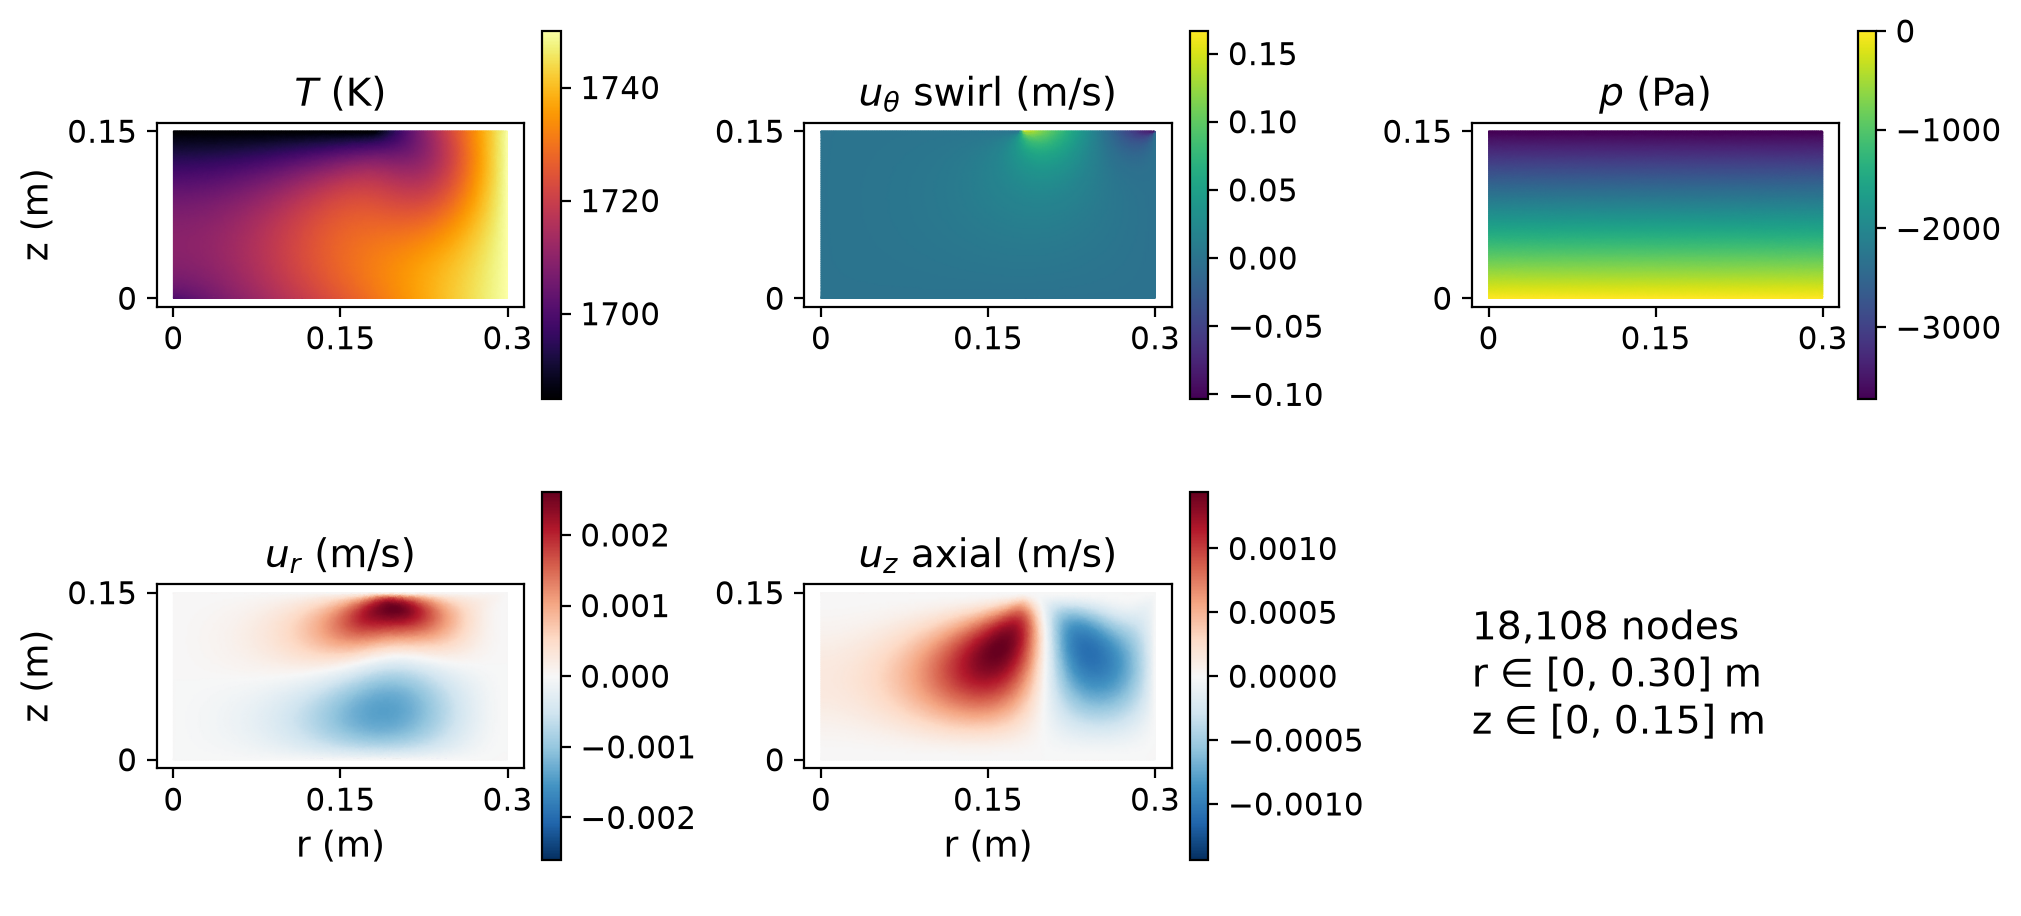
\includegraphics[width=\linewidth]{data_fields.png}
\figcap{Training data: $T$, swirl $u_\theta$, $p$, radial $u_r$ and axial $u_z$. Note the counter-rotating cells and the thin swirl layer under the crystal.}
\end{columns}
\takeaway{Five fields spanning six orders of magnitude, from mm/s flow to kPa pressure.}
\end{frame}

\begin{frame}{Protocol and compute pipeline}
\begin{columns}[T,onlytextwidth]
\column{0.50\textwidth}
\begin{itemize}\footnotesize\setlength{\itemsep}{1pt}
  \item \textbf{Ablations:} classical-only at matched budget; random features in place of the PQC.
  \item \textbf{Baselines:} classical PINN and PINO, matched optimiser, sampling and seeds.
  \item \textbf{Generalisation:} hold out a whole operating condition.
  \item \textbf{Reporting:} per-field errors, unweighted loss terms, wall time.
\end{itemize}
\begin{center}
\footnotesize
\begin{tabular}{lll}
\toprule
Sweep & Range & Held out \\
\midrule
$T_{\mathrm{hot}}$ & 1730--1785\,K & 1780\,K \\
$\omega_c$ (crucible) & $-10$ to $-1$ rpm & $-4$ rpm \\
$\omega_s$ (crystal) & 4--20 rpm & 7 rpm \\
\bottomrule
\end{tabular}
\end{center}
\column{0.47\textwidth}
\centering
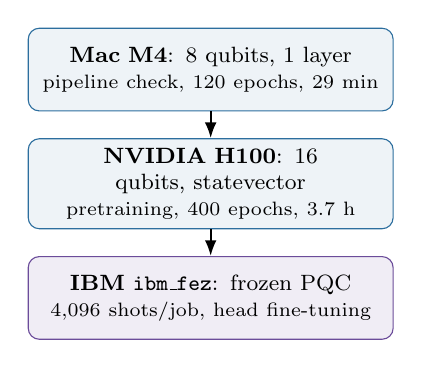
\begin{tikzpicture}[font=\footnotesize,
  st/.style={rounded corners,draw=cblue,fill=cblue!8,minimum width=4.6cm,minimum height=1.05cm,align=center,text width=4.4cm},
  sq/.style={rounded corners,draw=qpurple,fill=qpurple!10,minimum width=4.6cm,minimum height=1.05cm,align=center,text width=4.4cm},
  arr/.style={-{Latex[length=2mm]},thick}]
\node[st] (a) at (0,0) {\textbf{Mac M4}: 8 qubits, 1 layer\\\scriptsize pipeline check, 120 epochs, 29 min};
\node[st] (b) at (0,-1.45) {\textbf{NVIDIA H100}: 16 qubits, statevector\\\scriptsize pretraining, 400 epochs, 3.7 h};
\node[sq] (c) at (0,-2.9) {\textbf{IBM \texttt{ibm\_fez}}: frozen PQC\\\scriptsize 4,096 shots/job, head fine-tuning};
\draw[arr] (a)--(b); \draw[arr] (b)--(c);
\end{tikzpicture}
\end{columns}
\takeaway{16 qubits are exactly simulable on one GPU: hardware runs test noise and deployment, not quantum advantage.}
\end{frame}

\begin{frame}{Result 1: fast convergence in the data-driven phase}
\begin{columns}[T,onlytextwidth]
\column{0.44\textwidth}
\begin{center}
\footnotesize
\begin{tabular}{llll}
\toprule
Epoch & Train loss & Val MSE & Val $T$ \\
\midrule
1  & $1.16\!\times\!10^{-2}$ & $4.83\!\times\!10^{-3}$ & $1.37\!\times\!10^{-3}$ \\
10 & $5.92\!\times\!10^{-5}$ & $3.11\!\times\!10^{-4}$ & $1.47\!\times\!10^{-4}$ \\
\textbf{20} & $\mathbf{5.26\!\times\!10^{-5}}$ & $\mathbf{1.58\!\times\!10^{-4}}$ & $\mathbf{5.07\!\times\!10^{-5}}$ \\
30 & $2.96\!\times\!10^{-5}$ & $1.75\!\times\!10^{-4}$ & $6.15\!\times\!10^{-5}$ \\
50 & $2.07\!\times\!10^{-5}$ & $2.13\!\times\!10^{-4}$ & $2.91\!\times\!10^{-5}$ \\
\bottomrule
\end{tabular}
\end{center}
\vspace{0.1cm}
\small Validation MSE drops \textbf{30$\times$ in 20 epochs}; best checkpoint $1.58\times10^{-4}$ (random spatial split).
\column{0.53\textwidth}
\centering
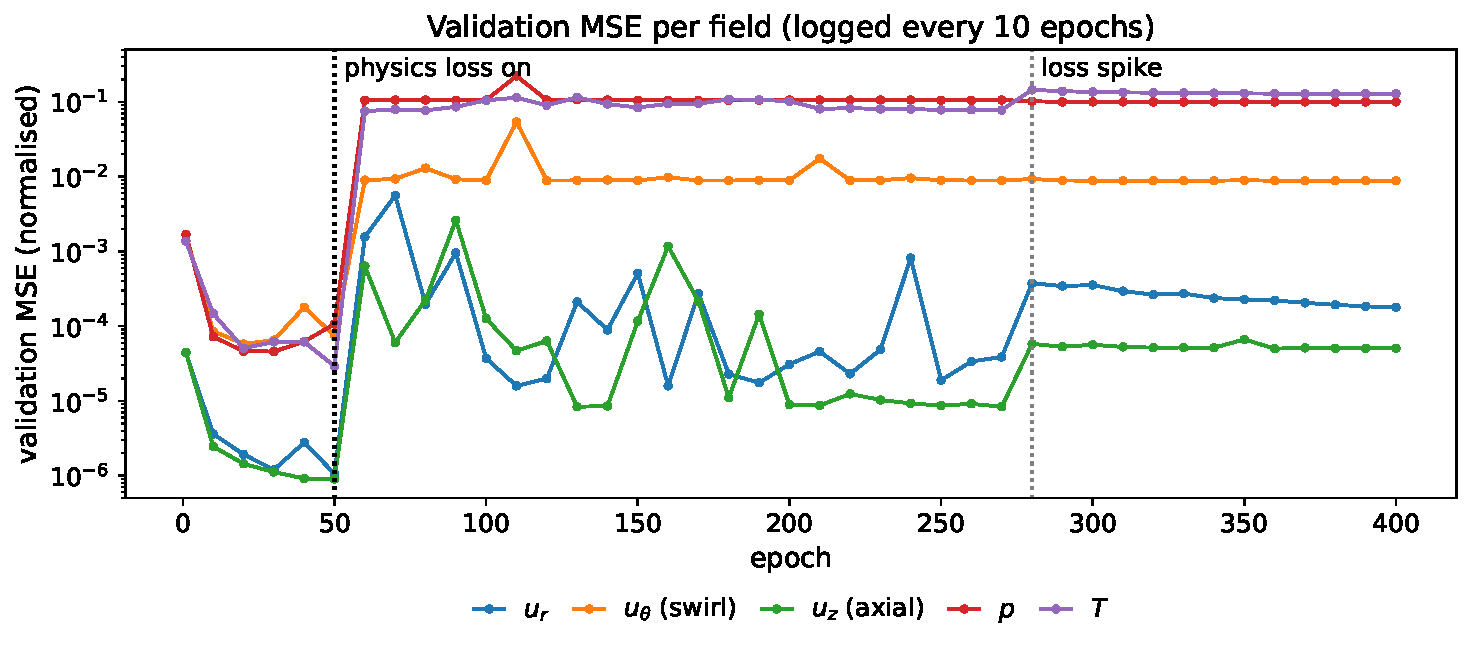
\includegraphics[width=\linewidth,height=0.64\textheight,keepaspectratio]{training_val_fields.pdf}
\figcap{Per-field validation MSE over 400 epochs; physics loss switches on at epoch 50.}
\end{columns}
\takeaway{Fast early convergence is measured; a matched classical baseline is the next test.}
\end{frame}

\begin{frame}{Result 2: temperature and swirl fields}
\centering
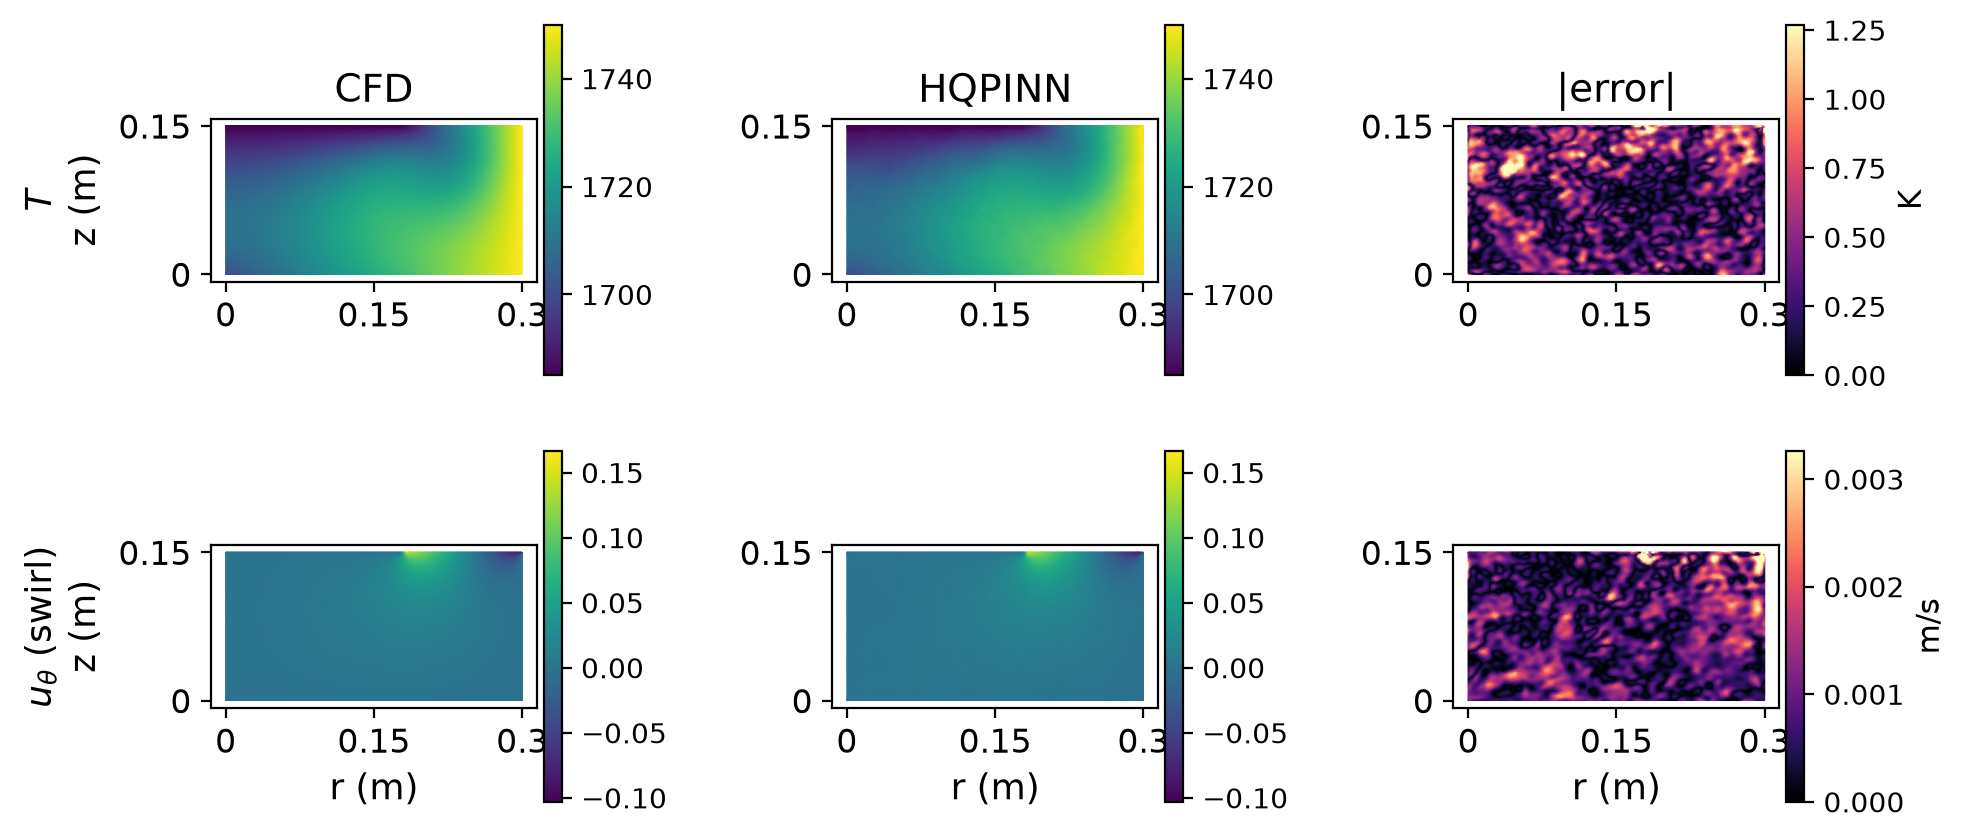
\includegraphics[width=0.86\linewidth,height=0.64\textheight,keepaspectratio]{field_maps_best_Tsw.png}
\figcap{CFD vs Hybrid-QPINN (best checkpoint) and absolute error: $T$ (error $\lesssim$1.25\,K on a 65\,K range) and $u_\theta$ (error $\lesssim3\times10^{-3}$\,m/s on $\pm0.15$\,m/s).}
\takeaway{The thin swirl layer under the crystal and the hot-wall thermal gradient are both reproduced.}
\end{frame}

\begin{frame}{Result 3: velocities, fields}
\begin{columns}[T,onlytextwidth]
\column{0.63\textwidth}
\centering
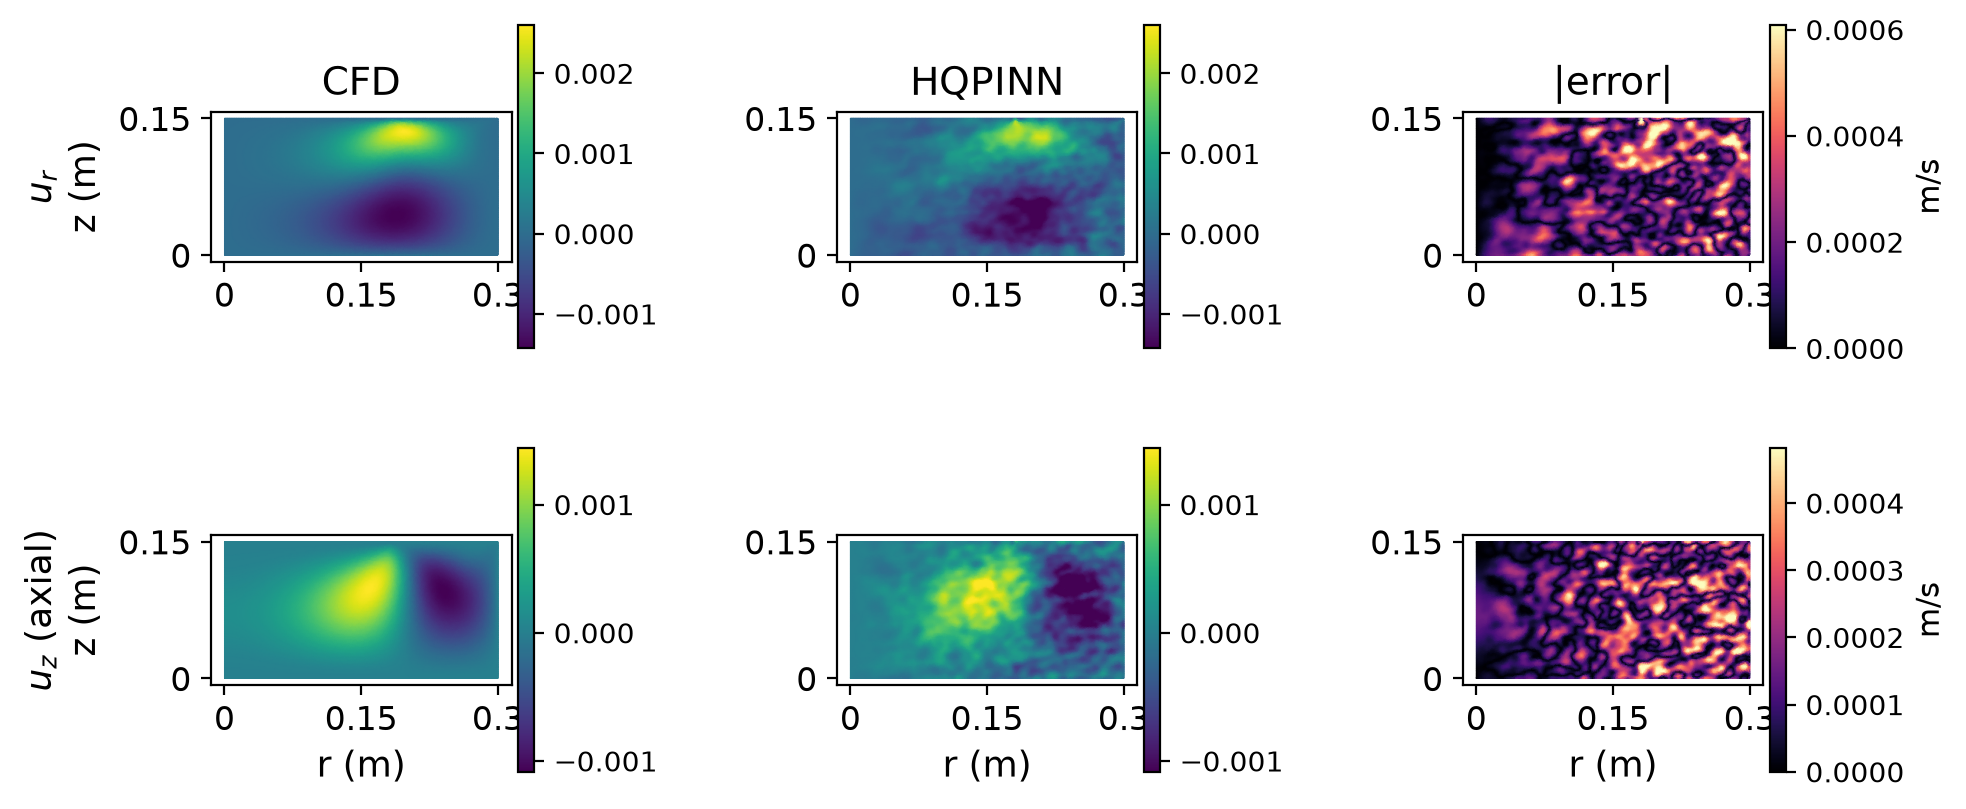
\includegraphics[width=\linewidth]{field_maps_best_urz.png}
\figcap{$u_r$ (top) and $u_z$ (bottom): CFD, Hybrid-QPINN, $|$error$|$.}
\column{0.34\textwidth}
\begin{center}
\footnotesize
\begin{tabular}{ll}
\toprule
Field & Val MSE (norm.) \\
\midrule
$u_r$ & $1.93\times10^{-6}$ \\
$u_z$ & $5.78\times10^{-5}$ \\
$u_\theta$ & $1.44\times10^{-6}$ \\
$p$ & $4.62\times10^{-5}$ \\
$T$ & $5.07\times10^{-5}$ \\
\bottomrule
\end{tabular}
\end{center}
\footnotesize Counter-rotating cells are located correctly; the remaining error is small-scale noise.
\end{columns}
\takeaway{All five coupled fields are fitted in distribution at the best checkpoint.}
\end{frame}

\begin{frame}{Result 4: naive physics weighting destabilises training}
\begin{columns}[T,onlytextwidth]
\column{0.52\textwidth}
\begin{center}
\footnotesize
\begin{tabular}{lllr}
\toprule
Field & Best (ep.\,20) & Final (ep.\,400) & Factor \\
\midrule
$u_r$ & $1.93\times10^{-6}$ & $1.79\times10^{-4}$ & 93$\times$ \\
$u_z$ & $5.78\times10^{-5}$ & $8.83\times10^{-3}$ & 153$\times$ \\
$u_\theta$ & $1.44\times10^{-6}$ & $5.06\times10^{-5}$ & 35$\times$ \\
$p$ & $4.62\times10^{-5}$ & $0.100$ & \textbf{2,165$\times$} \\
$T$ & $5.07\times10^{-5}$ & $0.129$ & \textbf{2,544$\times$} \\
\bottomrule
\end{tabular}
\end{center}
{\scriptsize\ttfamily
{[0280]} loss=1.04e+09 data=5.06e-02 phys=2.16e+10\\
{[0290]} loss=1.18e+14 data=4.97e-02 phys=2.15e+15}
\column{0.44\textwidth}
\begin{alertblock}{Diagnosis}
\small Data loss stays near 0.05; the blow-up is entirely in the physics residual, caused by the $p_{\mathrm{coeff}}$ scale mismatch (Bottleneck 3).
\end{alertblock}
\begin{exampleblock}{Fixes under test}
\small Physics weight 0.001--0.005; per-field pressure scaling.
\end{exampleblock}
\end{columns}
\takeaway{A classical-side issue, not a quantum one: the PQC is detached from the physics loss.}
\end{frame}

\begin{frame}{Result 5: the circuit on real quantum hardware}
\begin{columns}[T,onlytextwidth]
\column{0.60\textwidth}
\centering
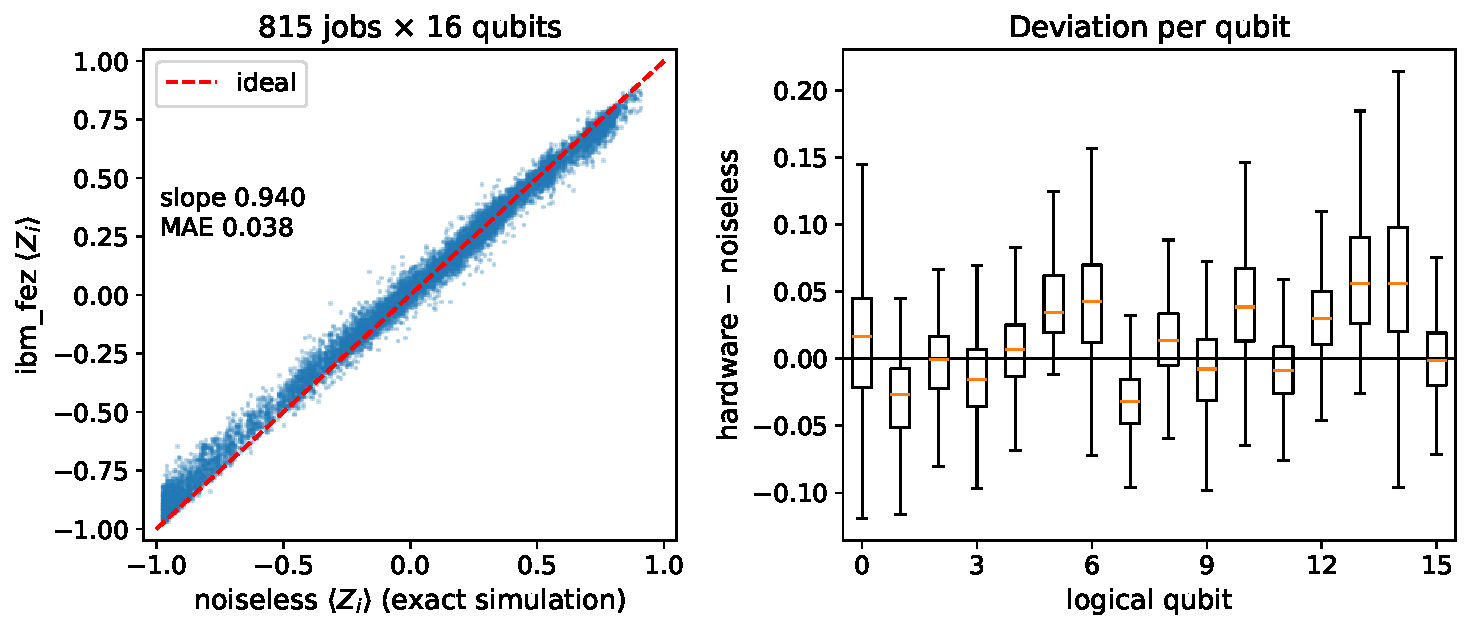
\includegraphics[width=\linewidth,height=0.58\textheight,keepaspectratio]{ibm_hw_vs_sim.pdf}
\figcap{\texttt{ibm\_fez} vs exact simulation, 815 jobs $\times$ 16 qubits: slope 0.940, MAE 0.038.}
\column{0.37\textwidth}
\begin{center}
\scriptsize
\begin{tabular}{ll}
\toprule
Fine-tuning session & Value \\
\midrule
Backend & \texttt{ibm\_fez} (156 qubits) \\
Jobs completed / failed & \textbf{500 / 0} \\
Shots per job & 4,096 \\
Session & 125 min \\
Trainable scope & head (19,205) \\
\bottomrule
\end{tabular}
\end{center}
\begin{block}{Reading}
\scriptsize Shot noise is at most 0.016, so the 0.038 gap is device noise (gates, readout), which shrinks $\langle Z\rangle$ toward 0 (slope $<1$).
\end{block}
\end{columns}
\takeaway{More shots will not close the gap; error mitigation and head re-adaptation will.}
\end{frame}

\begin{frame}{Inside the trained circuit}
\begin{columns}[T,onlytextwidth]
\column{0.58\textwidth}
\centering
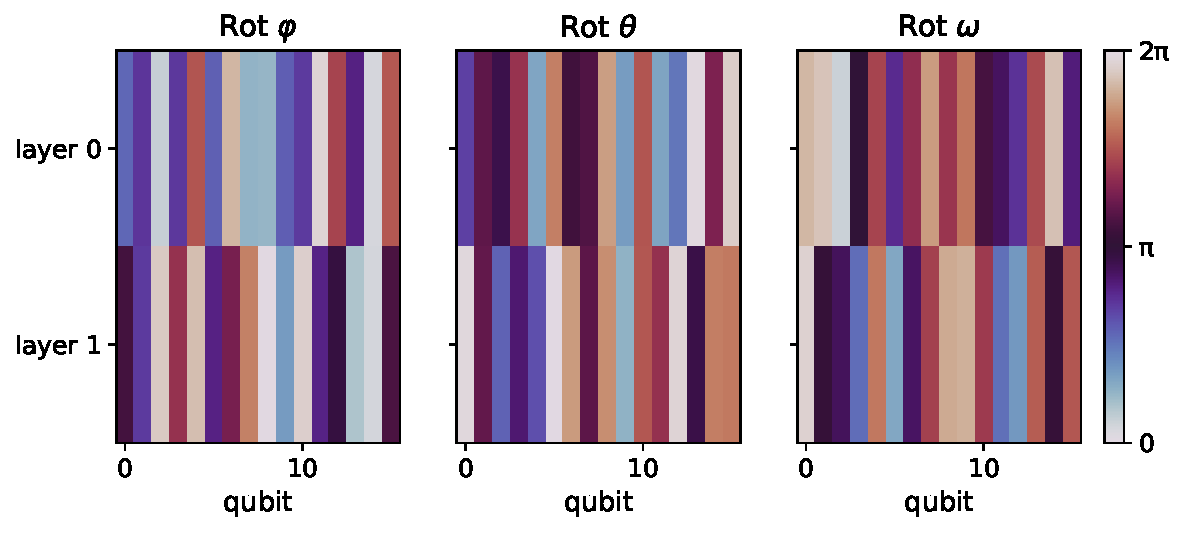
\includegraphics[width=\linewidth,height=0.56\textheight,keepaspectratio]{quantum_weights_heatmap.pdf}
\figcap{Trained Rot angles $(\varphi,\vartheta,\omega)$ per qubit, layers 0 and 1.}
\column{0.39\textwidth}
\begin{itemize}\small\setlength{\itemsep}{3pt}
  \item Angles span the full $[0,2\pi]$ range (mean 3.49, std 1.79 rad).
  \item No qubit stuck at a degenerate value; the two layers learn different patterns.
  \item LayerNorm weights qubits unequally ($\gamma\approx0.3$--$1.2$) in longer runs.
\end{itemize}
\end{columns}
\takeaway{The circuit is active and differentiated; whether it adds accuracy is for the ablation to decide.}
\end{frame}

\begin{frame}{Generalisation baseline: classical surrogate on unseen conditions}
\begin{columns}[T,onlytextwidth]
\column{0.44\textwidth}
\begin{block}{Gaussian-process surrogate}
\scriptsize Learns $(r,z,s)\mapsto$ fields; one whole case per sweep held out. NRMSE = RMSE / field std.
\end{block}
\centering
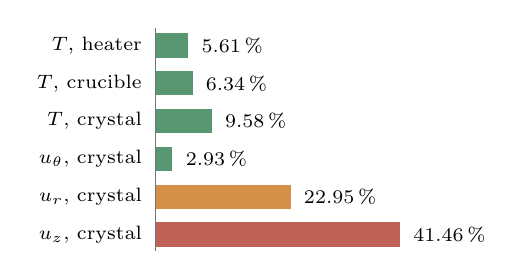
\begin{tikzpicture}[x=0.075cm,y=0.48cm,font=\scriptsize]
\foreach \lab/\val/\col [count=\i] in {%
  {$T$, heater}/5.61/okgreen,
  {$T$, crucible}/6.34/okgreen,
  {$T$, crystal}/9.58/okgreen,
  {$u_\theta$, crystal}/2.93/okgreen,
  {$u_r$, crystal}/22.95/warnorange,
  {$u_z$, crystal}/41.46/qred}{%
  \fill[\col!80] (0,-\i-0.32) rectangle (\val,-\i+0.32);
  \node[anchor=east] at (-0.6,-\i) {\lab};
  \node[anchor=west] at (\val+0.6,-\i) {\val\,\%};
}
\draw[phgray] (0,-0.55)--(0,-6.45);
\end{tikzpicture}
\column{0.53\textwidth}
\centering
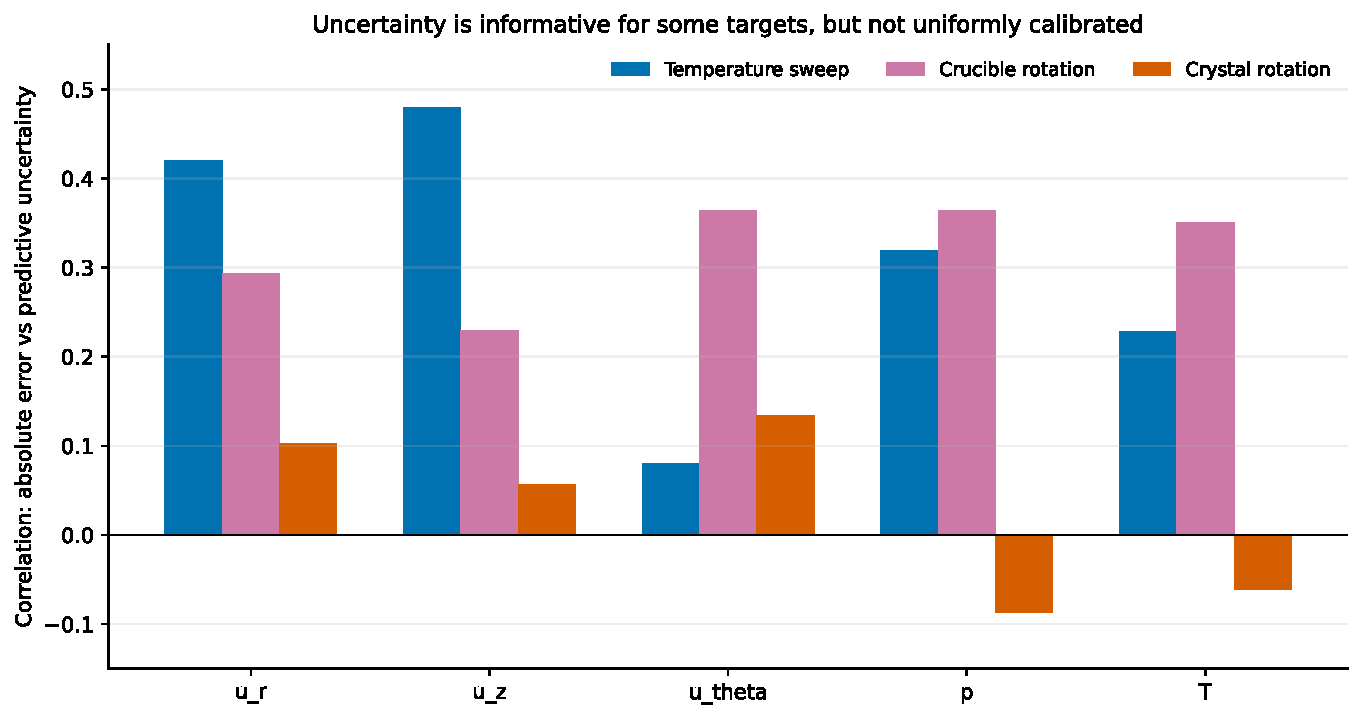
\includegraphics[width=\linewidth,height=0.53\textheight,keepaspectratio]{gpr_uncertainty.pdf}
\figcap{Correlation between GPR predictive uncertainty and actual error, per field and sweep.}
\end{columns}
\takeaway{$T$ generalises (5.6--9.6\%), velocities do not (23--41\%): the bar QPINO must beat.}
\end{frame}

% =====================================================================
\section{Outlook}
% =====================================================================

\begin{frame}{Current status}
\renewcommand{\arraystretch}{1.1}
\small
\begin{tabular}{p{0.44\textwidth} p{0.50\textwidth}}
\toprule
\multicolumn{2}{l}{\textcolor{okgreen}{\textbf{Measured so far}}} \\
\midrule
Hybrid pipeline runs on GPU and real QPU & 500/500 IBM jobs; MAE 0.038 vs simulation \\
Five coupled CZ fields fitted & Val MSE $1.58\times10^{-4}$, 30$\times$ drop in 20 epochs \\
Physics loss needs field-aware scaling & 2,000$\times$ degradation for $p$ and $T$ \\
\midrule
\multicolumn{2}{l}{\textcolor{warnorange}{\textbf{Still to be tested}}} \\
\midrule
Faster convergence than PINN/PINO & Match the classical baseline \\
PQC adds accuracy over classical features & Classical-only and random-feature ablations \\
Sharper generalisation & Case-wise holdout vs GPR / PINO (QPINO) \\
Reduced computational cost & GPU-hours to target error \\
Concentration, interfaces, LH$_2$ & Species equation, interface tracking \\
\bottomrule
\end{tabular}
\takeaway{Early indications are positive; matched ablations will decide the hybrid-vs-classical question.}
\end{frame}

\begin{frame}{Next benchmark: LH$_2$ cryogenic boil-off}
\begin{columns}[T,onlytextwidth]
\column{0.55\textwidth}
\begin{block}{Physics to capture}
\begin{itemize}\small
  \item Wall heat leak $\to$ natural-convection boundary layer and thermal stratification.
  \item Turbulent convection (RANS in the reference CFD).
  \item Liquid--vapour interface with evaporation (VOF + phase change).
  \item Outputs: velocity, temperature, phase fraction, boil-off rate, ullage pressure.
\end{itemize}
\end{block}
\column{0.41\textwidth}
\centering
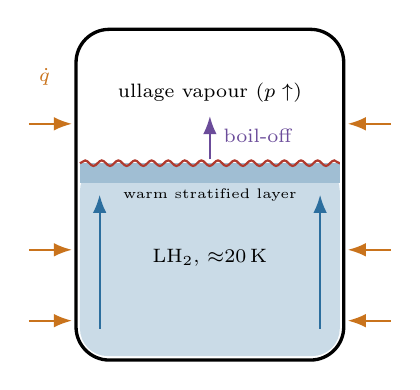
\begin{tikzpicture}[font=\scriptsize]
\draw[very thick,rounded corners=12pt] (0,0) rectangle (3.4,4.2);
\fill[cblue!25,rounded corners=10pt] (0.05,0.05) rectangle (3.35,2.5);
\fill[cblue!45] (0.05,2.25) rectangle (3.35,2.5);
\draw[qred,thick,decorate,decoration={snake,amplitude=1pt,segment length=6pt}] (0.05,2.5)--(3.35,2.5);
\node at (1.7,3.4) {ullage vapour ($p\uparrow$)};
\node at (1.7,1.3) {LH$_2$, $\approx$20\,K};
\node[font=\tiny] at (1.7,2.1) {warm stratified layer};
\foreach \y in {0.5,1.4,3.0}{\draw[-{Latex},warnorange,thick] (-0.6,\y)--(-0.05,\y);\draw[-{Latex},warnorange,thick] (4.0,\y)--(3.45,\y);}
\node[warnorange] at (-0.4,3.6) {$\dot q$};
\draw[-{Latex},thick,qpurple] (1.7,2.55)--(1.7,3.1);
\node[qpurple,anchor=west] at (1.75,2.85) {boil-off};
\draw[-{Latex},cblue,thick] (0.3,0.4)--(0.3,2.1);
\draw[-{Latex},cblue,thick] (3.1,0.4)--(3.1,2.1);
\end{tikzpicture}
\end{columns}
\takeaway{Same framework, harder physics: turbulence plus a moving phase boundary.}
\end{frame}

\begin{frame}{Real-time digital twins}
\centering
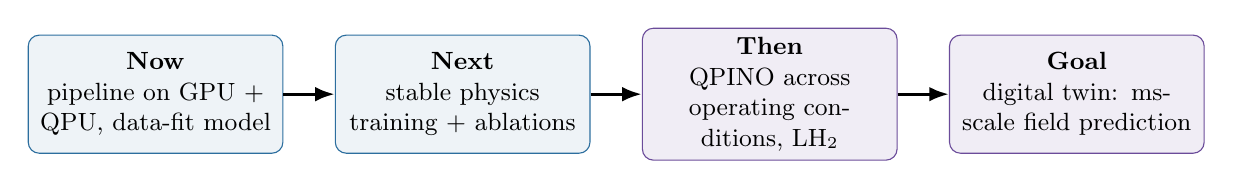
\begin{tikzpicture}[
  font=\small,
  st/.style={rounded corners,draw=cblue,fill=cblue!8,minimum width=3.2cm,minimum height=1.5cm,align=center,text width=3.0cm},
  sq/.style={rounded corners,draw=qpurple,fill=qpurple!10,minimum width=3.2cm,minimum height=1.5cm,align=center,text width=3.0cm},
  arr/.style={-{Latex[length=2.5mm]},very thick}
]
\node[st] (a) at (0,0) {\textbf{Now}\\pipeline on GPU + QPU, data-fit model};
\node[st] (b) at (3.9,0) {\textbf{Next}\\stable physics training + ablations};
\node[sq] (c) at (7.8,0) {\textbf{Then}\\QPINO across operating conditions, LH$_2$};
\node[sq] (d) at (11.7,0) {\textbf{Goal}\\digital twin: ms-scale field prediction};
\draw[arr] (a)--(b); \draw[arr] (b)--(c); \draw[arr] (c)--(d);
\end{tikzpicture}

\vspace{0.4cm}
\begin{block}{QPINO: one model for the whole process window}
\small Process parameters become inputs:\quad $(r,z,s)\mapsto(u_r,u_z,u_\theta,p,T)$,\quad $s\in\{T_{\mathrm{hot}},\omega_c,\omega_s,v_{\mathrm{pull}}\}$.\\
Trained once on CFD cases (generated by agentic CFD, AutoFOAM), then queried for any setting.
\end{block}
\takeaway{Inference needs no QPU: the trained 16-qubit circuit is evaluated in milliseconds on a GPU.}
\end{frame}

\begin{frame}{Key takeaways}
\begin{enumerate}\setlength{\itemsep}{5pt}
  \item \textbf{Problem:} classical PINNs struggle with spectral bias, loss imbalance and field-scale mismatch in coupled transport.
  \item \textbf{Model:} Fourier features + data re-uploading + a shallow 16-qubit PQC (96 angles) as a trainable feature map, built with PennyLane and Qiskit.
  \item \textbf{Results:} all five coupled CZ fields fitted (val MSE $1.58\times10^{-4}$); the circuit runs on IBM hardware (500/500 jobs, MAE 0.038).
  \item \textbf{Next:} matched ablations for convergence, generalisation and cost; QPINO for crystal growth and LH$_2$ digital twins.
\end{enumerate}
\end{frame}

\begin{frame}{References}
\scriptsize
\begin{itemize}\setlength{\itemsep}{1pt}
  \item Raissi, Perdikaris, Karniadakis, \emph{Physics-informed neural networks}, J.\ Comput.\ Phys.\ (2019).
  \item Rahaman et al., \emph{On the spectral bias of neural networks}, ICML 2019.
  \item Tancik et al., \emph{Fourier features let networks learn high frequency functions}, NeurIPS 2020.
  \item P\'erez-Salinas et al., \emph{Data re-uploading for a universal quantum classifier}, Quantum (2020).
  \item Schuld, Sweke, Meyer, \emph{Effect of data encoding on the expressive power of variational quantum machine-learning models}, PRA (2021).
  \item Wang, Teng, Perdikaris, \emph{Understanding and mitigating gradient pathologies in PINNs}, SIAM J.\ Sci.\ Comput.\ (2021).
  \item Li et al., \emph{Physics-informed neural operator for learning PDEs} (2021).
  \item Bergholm et al., \emph{PennyLane: automatic differentiation of hybrid quantum-classical computations}, arXiv:1811.04968.
  \item Javadi-Abhari et al., \emph{Quantum computing with Qiskit}, arXiv:2405.08810.
  \item Huang, Cao, Liu, Liu, \emph{Thermal-fluid coupling in Czochralski silicon growth based on an improved PINN}, AIP Advances 15, 105202 (2025).
  \item Chapagain et al., \emph{Component-level evaluation of adaptive PINN training for CFD-oriented crystal growth simulation}, NeurIPS 2026 Sim2Science workshop.
  \item Neelan, Seshaditya, \emph{AutoFOAM: the self-refining autonomous OpenFOAM agent}.
\end{itemize}
\end{frame}

\begin{frame}
\centering
\Large\textbf{Thank you}

\vspace{0.3cm}
\normalsize Questions?

\vspace{0.6cm}
\footnotesize
\textbf{Acknowledgements:} Niruta Chapagain, Rohit Raj (adaptive PINN study);
Bertwin Kurisinkal Shine, TU Chemnitz (CZ reference CFD);
Arun Govind Neelan (SciM); Quasi AI Team \& Co.
\end{frame}

\end{document}
